% Niveau :      PCSI *
% Discipline :  Chimie Orga I
% Mots clés :   Spectrométrie UV-visible, Réactions acidobasiques

\begin{exercise}{\'Etude des thiocyanates}{2}{PCSI}
{Chimie générale,Réactions de complexation}{bermu}

\begin{questions}
\questioncours Structure et stabilité des complexes en solution aqueuse. \\ On définira les constantes de formation.

\begin{EnvUplevel}
    On s'intéresse à présent aux complexes formés par les ions thiocyanates SCN$^{-}$ et cuivre (II). Leur diagramme de distribution en fonction de pSCN $=-\log\dfrac{\mathrm{[SCN]}}{c^\circ}$ (où $c^\circ = 1$~M) est donné ci-dessous : \vspace{-.5em}
    
    \begin{figure}[H]
        \centering
        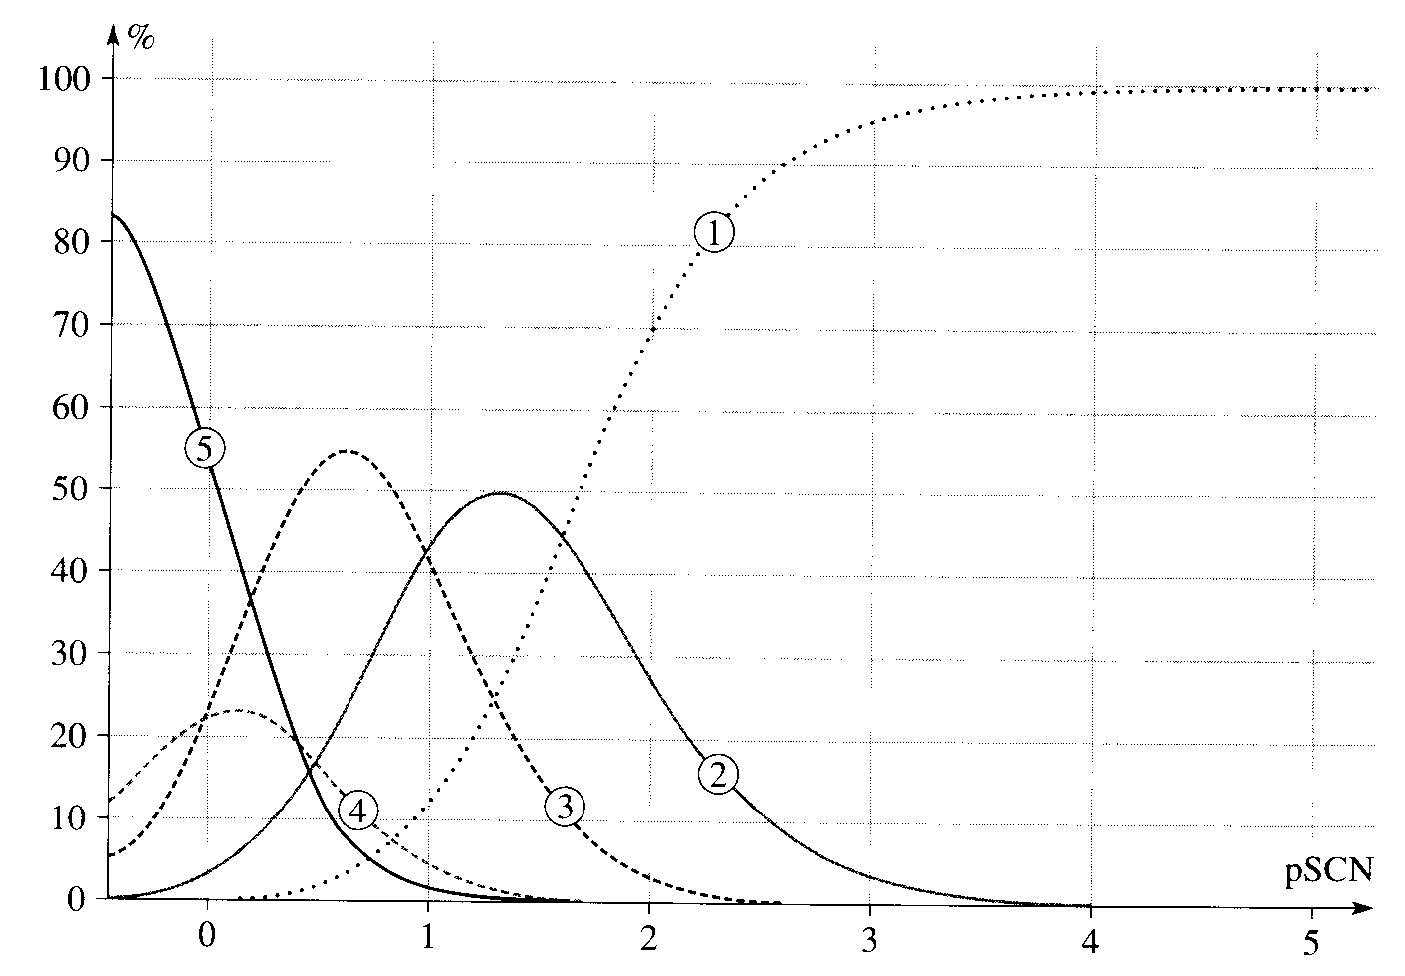
\includegraphics[width=.9\linewidth]{chimiePC/gene/thio.jpg}\vspace{-1.3em}
        \caption{Diagramme de distribution de complexes entre Cu$^{2+}$ et SCN$^{-}$.} \vspace{-0.8em}
    \end{figure}
\end{EnvUplevel}

\question Le numéro atomique du cuivre est $Z = 29$. En déduire la position de cet élément dans le tableau périodique (numéro de ligne, numéro de colonne) en justifiant la réponse. Donner la configuration électronique de l’ion Cu$^{2+}$.

\question Montrer que le ligand thiocyanate SCN$^{-}$ peut être écrit selon deux formes mésomères de représentativité proche. \\
Expliquer alors pourquoi on qualifie ce ligand de ligand ambidenté, et non pas de ligand bidenté.

\question Donner la formule et la nomenclature du complexe correspondant à chacune des courbes.

\question Déterminer les constantes de formation successives p$K_{fi}$ de ces complexes en justifiant la méthode utilisée.

\question Le complexe correspondant à la courbe 4 a une forte tendance à la dismutation. À quoi le voit-on sur le diagramme de distribution ? \\
Écrire l'équation chimique qui rende compte de ce phénomène et calculer sa constante d’équilibre. \\
Justifier rapidement que ce complexe soit peu stable comparé aux autres.

\begin{EnvUplevel}
    On constitue une solution aqueuse de 250 mL en dissolvant 10 mmol de sulfate de cuivre CuSO$_4$ et 1,0 mmol de thiocyanate de potassium KSCN.
\end{EnvUplevel}

\question{\sffamily Question ouverte :} En faisant les approximations nécessaires, donner les réactions chimiques qui ont lieu et décrire le système chimique à l'équilibre.

\end{questions}

\paragraph{Données : }~\\
L’indice de coordination du complexe Cu$^{2+}$ / SCN$^{-}$ varie de 1 à 4.

\end{exercise}

\begin{solution}

\begin{questions}
    \stepcounter{question}

    \question En appliquant les règles de remplissage :
    $$\mathrm{[Cu]} : 1s^2 2s^2 2p^6 3s^2 3p^6 4s^2 3d^9,$$
    {\sffamily Remarque :} dans le cas du cuivre, par la règle de Hund, il est plus facile d'avoir la configuration de valence $4s^1 3d^10$ car les énergies de la $4s$ et la $3d$ sont proches.
    
    Le cuivre est donc dans la 4ème période ($4s$) et le cuivre est dans la 11ème colonne $4s^2 3d^9$.
    
    $$\text{Ainsi la configuration de Cu}^{2+} \text{ est } \quad 1s^2 2s^2 2p^6 3s^2 3p^6 4s^0 3d^9.$$
    
    \question\hfill
    \schemestart
        \chemfig{@{a1}{^\ominus\hspace{1ex}\lewis{246,S}}-[@{a2},1.3]C~[@{b1},1.1]@{b2}\lewis{0,N}}
        \chemmove[red,-stealth,red,shorten >=3pt]{
            \draw(a1)..controls +(up:5mm) and +(north west:2mm).. (a2);}
        \chemmove[red,-stealth,red,shorten <=2pt]{
            \draw(b1)..controls +(up:5mm) and +(north west:2mm).. (b2);}
        \arrow{<->}[,1.5]
        \chemfig{\lewis{35,S}=[,1.1]C=[,1.3]\lewis{17,N}\hspace{1ex}^\ominus}
    \schemestop\chemnameinit{}\hfill~
    
    Le soufre et l’azote sont d’électronégativités voisines et donc ces deux formules mésomères sont de représentativités proches : la charge négative est à peu près équitablement répartie entre  N et S. L’ion SCN$^{-}$ peut donc se lier par S ou bien par N, mais pas simultanément puisque l’ion est linéaire (VSEPR AX$_2$), d'où la qualification d'ambidente.
    
    \question \`A haut pSCN (très bas [SCN]), il n'y a que Cu$^{2+}$, ainsi :
    \begin{enumerate}
        \item ~Cu$^{2+}$, ion cuivre II ;
        \item ~[CuSCN]$^+$, ion thiocyanatocuivre II ;
        \item ~[Cu(SCN)$_2$], dithiocyanatocuivre II ;
        \item ~[Cu(SCN)$_3$]$^{-}$, trithiocyanatocuprate II ;
        \item ~[Cu(SCN)$_4$]$^{2-}$, tetrathiocyanatocuprate II.
    \end{enumerate}
    
    \question p$K_{fi}$ est la constante de la réaction $[\mathrm{Cu(SCN)}_{i-1}]^{3-i} + \mathrm{[SCN^-]} \longrightarrow [\mathrm{Cu(SCN)}_i]^{2-i}$ donc
    $$\text{pSCN} = \log K_{fi} + \log\dfrac{[\mathrm{Cu(SCN)}_{i-1}]^{3-i}}{[\mathrm{Cu(SCN)}_i]^{2-i}}.$$
    \`A l'intersection des courbes $i$ et $i+1$, on a $[\mathrm{Cu(SCN)}_{i-1}]^{3-i} = [\mathrm{Cu(SCN)}_i]^{2-i}$ soit pSCN = $\log K_{fi}$.
    
    Donc $K_{f1} = 10^{1,6}$, $K_{f2} = 10^{1}$, $K_{f3} = 10^0$, $K_{f4} = 10^{0,4}$ (! intersection 4-5 !).
    
    \question La dismutation s'écrit $\mathrm{2[Cu(SCN)_3]^- \leftrightharpoons [Cu(SCN)_2] + [Cu(SCN)_4]^{2-}}$, de constante $K = \dfrac{K_{f4}}{K_{f3}} = 10^{0,4} > 1$ thermodynamiquement favorisée (on forme 4 et on détruit 3).
    
    Cela est dû au fait que la coordination $n=3$ n'est pas favorisée (cf. config électronique)
    
    \question [Cu$^2+$]$ = 40$ mM et [SCN$^-$]$ = 4,0$ mM, soit pSCN$ = 2,4$. Donc d'après le schéma les espèces prédominantes sont [Cu$^{2+}$] et [SCN$^-$] et la réaction prépondérante sera :
    \begin{center}\begin{tabularx}{9cm}{r|C|C|C}
&
\multicolumn{1}{|c!{\makebox[0pt]{+}}}{Cu$^{2+}$}
&
\multicolumn{1}{c!{\makebox[0pt]{$\leftrightharpoons$}}}{SCN$^-$}
&
[CuSCN]$^-$
\\
\hline\hline
Init. & $c_1$ & $c_2$ & 0 \\
Eq. & $c_1 - \xi$ & $c_2 - \xi$ & $\xi$
\end{tabularx}\end{center}
    $$\text{pour laquelle :}\qquad K_{f1} = \dfrac{\xi}{(c_1 - \xi)(c_2 - \xi)} \qquad \Longleftrightarrow \qquad \xi \simeq 2,2 \text{ mM}.$$
    
Ensuite pour les autres espèces, l'avancement des $fi$ sera négligeable et on aura pour $i > 1$, \vspace{-.8em}
$$[\mathrm{Cu(SCN)}_i]^{2-i} = K_{fi} [\mathrm{SCN}^{-1}] [\mathrm{Cu(SCN)}_{i-1}]^{3-i},$$
et donc, en définitive :
\begin{itemize}
    \item $[\mathrm{Cu}^{2+}] = 3,8 \times 10^{-2} \text{ M}$ ;
    \item $[\mathrm{SCN}^-] = 1,8 \times 10^{-3} \text{ M}$ ;
    \item $[\mathrm{CuSCN}^-] = 2,2 \times 10^{-3} \text{ M}$ ;
    \item $[\mathrm{Cu(SCN)}_2] = 3,6 \times 10^{-5} \text{ M}$ ;
    \item $[\mathrm{Cu(SCN)}_3]^- = 5,8 \times 10^{-8} \text{ M}$ ;
    \item $[\mathrm{Cu(SCN)}_4]^{2-} = 2,6 \times 10^{-10} \text{ M}$ ;
\end{itemize}
    
    
    
\end{questions}
\end{solution}